% !TEX root = Eco-Model.tex
\section{Experiment and result Analysis} % (fold)
\label{sec:Experiment_results}

Entities in the manufacturing ecosystem we designed above have these traits, they are: \begin{inparaenum}
\item autonomous and self-directed, 
\item social, interacting with other entities, 
\item controlled by the environment, 
\item self-contained.
\end{inparaenum} They optimize their multi-objective decision makings to interact with others and the environment, hence, agent-based modeling and simulation(ABMS) technique\cite{Macal2009,north2007managing} is suitable for the study of the complex system. With the help of Repast Simphony\cite{North2013} package, we realized the ecosystem model and performed some experiments on it.
\subsection{Agent-based modeling and simulation design} % (fold)
\label{sub:agent_based_modeling_and_simulation}
\subsubsection{Model realization}
\begin{asparaenum}
\item Main agents
\suspend{asparaenum}
\begin{figure}[htbp]
\centering
\tiny
\subfloat[Job related classes]{\begin{tikzpicture}
    % !TEX root = flow_head.tex

\begin{class}[text width=8cm]{Job}{0,0}
	\attribute{+ allocated: boolean}
	\attribute{+ allocation: Map}
	\attribute{+ candidates: Map}
	\attribute{+ inNeed: boolean}
	\attribute{+ needResourceCapacity: Map}
	\attribute{+ predecessor: Set}
	\attribute{+ prepareStatus: Map}
	\attribute{- processBehavior: ProcessBehavior}
	\attribute{- selectBehavior: SelectBehavior}
	\operation{+ addCandidates(competitor: Machine): void}
	\operation{+ CheckStatus(): void}
	\operation{+ Need(): void}
	\operation{+ Review(m: Machine): void}
	\operation{+ Select(watchedAgent: Job): void}
\end{class}


    % !TEX root = flow_head.tex

\begin{class}[text width=8cm]{Task}{0,0}
	\attribute{+ master: Order}
	\attribute{+ owner: Map}
	\attribute{+ pause: boolean}
	\attribute{+ processingTime: int}
	\attribute{+ remainingTime: int}
	\attribute{+ type: Strihng}
	\operation{+ Task()}
	\operation{+ addOwner(user: User, p: int): void}
	\operation{+ CheckStatus(): void}
	\operation{+ Process(watchedAgent: Task): void}
	\operation{+ setParameters(taskData: Map): void}
\end{class}
    % !TEX root = flow_head.tex

\begin{class}[text width=.225\textwidth]{ServiceCall}{1.08,-3.7}
	\inherit{Job}
	\attribute{+ owner: Provider}
	\attribute{+ type: String}
	\operation{+ ServiceCall()}
	\operation{+ setParameter(scData: Map): void}
	\operation{+ Recall(): void}
\end{class}
    \end{tikzpicture}
    \label{fig:jobclassed}}\hspace{1pt}
\subfloat[Machine related classes]{\begin{tikzpicture}
    % !TEX root = flow_head.tex

\begin{class}[text width=.45\textwidth]{Machine}{0,0}
	\attribute{+ assignBehavior: AssignBehavior}
	\attribute{+ buffer: List}
	\attribute{+ competeList: List}
	\attribute{+ jobList: List}
	\attribute{+ owner: Provider}
	\attribute{+ releaseBehavior: ReleaseBehavior}
	\attribute{+ responseBehavior: ResponseBehavior}
	\attribute{+ responseList: List}
	\attribute{+ type: String}
	\operation{+ Assign(t: Task): void}
	\operation{+ Release(j: Job): void}
	\operation{+ Reply(watchedAgent: Job): void}
	\operation{+ Response(watchedAgent: Task): void}
	\operation{+ Review(j: Job):void}
\end{class}


    % !TEX root = flow_head.tex

\begin{class}[text width=.45\textwidth]{Resource}{-2.4,-3.66}
	\inherit{Machine}
	\attribute{+ available: int}
	\attribute{+ capacity: int}
	\attribute{+ master: Map}
	\attribute{+ needCap: Map}
	\attribute{+ sourceable: int}
	\operation{+ Resource()}
	\operation{+ addMaster(ser: Service, amonut: int): void}
	\operation{+ Assign(sc: ServiceCall, amount: int): void}
	\operation{+ Response(watchedAgent: ServiceCall): void}
\end{class}
    % !TEX root = flow_head.tex

\begin{class}[text width=.45\textwidth]{Service}{2.4,-3.66}
	\inherit{Machine}
	\attribute{+ resourceComposition: Map}
	\operation{+ Service()}
	\operation{+ OutSource(): void}
\end{class}
    \end{tikzpicture}
    \label{fig:machineclassed}}\\
\subfloat[User related classes]{\begin{tikzpicture}
    % !TEX root = flow_head.tex

\begin{class}[text width=.45\textwidth]{User}{0,0}
	\attribute{- agentIDCounter: long}
	\attribute{\# agentID: String}
\end{class}
    % !TEX root = flow_head.tex

\begin{class}[text width=.45\textwidth]{Provider}{-2.4,-1.2}
	\inherit{User}
	\attribute{+ candidates: List}
	\attribute{+ rank: double}
	\attribute{+ resourceList: List}
	\attribute{+ serviceList: List}
	\operation{+ GenerateResource(): void}
	\operation{+ GenerateService(serviceData: List): void}
	\operation{+ GenerateServiceCall(): void}
	\operation{+ RemoveServiceCall(sc: ServiceCall): void}
	
\end{class}
% !TEX root = flow_head.tex

\begin{class}[text width=.45\textwidth]{Demander}{2.4,-1.2}
	\inherit{User}
	\attribute{+ orderList: List}
	\attribute{+ taskMap: Map}
	\operation{+ GenerateOrder(orderID: String): void}
	\operation{+ ReadData(orderID: String): void}
\end{class}


    \end{tikzpicture}\label{fig:userclassed}}\hspace{3pt}
\subfloat[Cloud Platform]{\begin{tikzpicture}
	% !TEX root = flow_head.tex

\begin{class}[text width=8cm]{CloudPlatform}{0,0}
	\attribute{- agentIDCounter: long}
	\attribute{\# agentID: String}
	\attribute{+ finishCount: int}
	\attribute{+ userList: List}
	\operation{+ CreateProvider(): void}
	\operation{+ CreateDemander(): void}
\end{class}


	\end{tikzpicture}\label{fig:platform}}
\end{figure}


% \begin{figure}[htbp]
% 	\centering
% 	\tiny
% 	\begin{tikzpicture}
% 	% !TEX root = flow_head.tex

\begin{class}[text width=8cm]{CloudPlatform}{0,0}
	\attribute{- agentIDCounter: long}
	\attribute{\# agentID: String}
	\attribute{+ finishCount: int}
	\attribute{+ userList: List}
	\operation{+ CreateProvider(): void}
	\operation{+ CreateDemander(): void}
\end{class}


% 	\end{tikzpicture}
% 	\caption{Cloud Platform}
% 	\label{fig:platform}
% \end{figure}
% % \resume{asparaenum}
% % \item User related
% % \suspend{asparaenum}
% \begin{figure}[htbp]
%     \centering
%     \tiny
%     \begin{tikzpicture}
%     % !TEX root = flow_head.tex

\begin{class}[text width=.45\textwidth]{User}{0,0}
	\attribute{- agentIDCounter: long}
	\attribute{\# agentID: String}
\end{class}
%     % !TEX root = flow_head.tex

\begin{class}[text width=.45\textwidth]{Provider}{-2.4,-1.2}
	\inherit{User}
	\attribute{+ candidates: List}
	\attribute{+ rank: double}
	\attribute{+ resourceList: List}
	\attribute{+ serviceList: List}
	\operation{+ GenerateResource(): void}
	\operation{+ GenerateService(serviceData: List): void}
	\operation{+ GenerateServiceCall(): void}
	\operation{+ RemoveServiceCall(sc: ServiceCall): void}
	
\end{class}
% % !TEX root = flow_head.tex

\begin{class}[text width=.45\textwidth]{Demander}{2.4,-1.2}
	\inherit{User}
	\attribute{+ orderList: List}
	\attribute{+ taskMap: Map}
	\operation{+ GenerateOrder(orderID: String): void}
	\operation{+ ReadData(orderID: String): void}
\end{class}


%     \end{tikzpicture}
%     \caption{User related classes}
%     \label{fig:userclassed}
% \end{figure}
% \resume{asparaenum}
% \item Job related
% \suspend{asparaenum}
% \begin{figure}[htbp]
%     \centering
%     \tiny
%     \begin{tikzpicture}
%     % !TEX root = flow_head.tex

\begin{class}[text width=8cm]{Job}{0,0}
	\attribute{+ allocated: boolean}
	\attribute{+ allocation: Map}
	\attribute{+ candidates: Map}
	\attribute{+ inNeed: boolean}
	\attribute{+ needResourceCapacity: Map}
	\attribute{+ predecessor: Set}
	\attribute{+ prepareStatus: Map}
	\attribute{- processBehavior: ProcessBehavior}
	\attribute{- selectBehavior: SelectBehavior}
	\operation{+ addCandidates(competitor: Machine): void}
	\operation{+ CheckStatus(): void}
	\operation{+ Need(): void}
	\operation{+ Review(m: Machine): void}
	\operation{+ Select(watchedAgent: Job): void}
\end{class}


%     % !TEX root = flow_head.tex

\begin{class}[text width=8cm]{Task}{0,0}
	\attribute{+ master: Order}
	\attribute{+ owner: Map}
	\attribute{+ pause: boolean}
	\attribute{+ processingTime: int}
	\attribute{+ remainingTime: int}
	\attribute{+ type: Strihng}
	\operation{+ Task()}
	\operation{+ addOwner(user: User, p: int): void}
	\operation{+ CheckStatus(): void}
	\operation{+ Process(watchedAgent: Task): void}
	\operation{+ setParameters(taskData: Map): void}
\end{class}
%     % !TEX root = flow_head.tex

\begin{class}[text width=.225\textwidth]{ServiceCall}{1.08,-3.7}
	\inherit{Job}
	\attribute{+ owner: Provider}
	\attribute{+ type: String}
	\operation{+ ServiceCall()}
	\operation{+ setParameter(scData: Map): void}
	\operation{+ Recall(): void}
\end{class}
%     \end{tikzpicture}
%     \caption{Job related classes}
%     \label{fig:jobclassed}
% \end{figure}
% \resume{asparaenum}
% \item Machine related
% \end{asparaenum}
% \begin{figure}[htbp]
%     \centering
%     \tiny
%     \begin{tikzpicture}
%     % !TEX root = flow_head.tex

\begin{class}[text width=.45\textwidth]{Machine}{0,0}
	\attribute{+ assignBehavior: AssignBehavior}
	\attribute{+ buffer: List}
	\attribute{+ competeList: List}
	\attribute{+ jobList: List}
	\attribute{+ owner: Provider}
	\attribute{+ releaseBehavior: ReleaseBehavior}
	\attribute{+ responseBehavior: ResponseBehavior}
	\attribute{+ responseList: List}
	\attribute{+ type: String}
	\operation{+ Assign(t: Task): void}
	\operation{+ Release(j: Job): void}
	\operation{+ Reply(watchedAgent: Job): void}
	\operation{+ Response(watchedAgent: Task): void}
	\operation{+ Review(j: Job):void}
\end{class}


%     % !TEX root = flow_head.tex

\begin{class}[text width=.45\textwidth]{Resource}{-2.4,-3.66}
	\inherit{Machine}
	\attribute{+ available: int}
	\attribute{+ capacity: int}
	\attribute{+ master: Map}
	\attribute{+ needCap: Map}
	\attribute{+ sourceable: int}
	\operation{+ Resource()}
	\operation{+ addMaster(ser: Service, amonut: int): void}
	\operation{+ Assign(sc: ServiceCall, amount: int): void}
	\operation{+ Response(watchedAgent: ServiceCall): void}
\end{class}
%     % !TEX root = flow_head.tex

\begin{class}[text width=.45\textwidth]{Service}{2.4,-3.66}
	\inherit{Machine}
	\attribute{+ resourceComposition: Map}
	\operation{+ Service()}
	\operation{+ OutSource(): void}
\end{class}
%     \end{tikzpicture}
%     \caption{Machine related classes}
%     \label{fig:machineclassed}
% \end{figure}
\resume{asparaenum}
\item Behavior interfaces and classes
\end{asparaenum}
% \begin{asparaenum}
% \item Assign behavior
% \suspend{asparaenum}
\begin{figure}[htbp]
    \centering
    \tiny
    \begin{tikzpicture}
    % !TEX root = flow_head.tex

\begin{interface}[text width=.45\textwidth]{AssignBehavior}{0,0}
	\operation{+ BufferEnterance(t: Task, m: Machine): boolean}
	\operation{+ Queue(j: Job, m: Machine): void}
	\operation{+ Buff(t: Task, m: Machine): void}
\end{interface}


    % !TEX root = flow_head.tex

\begin{interface}[text width=.45\textwidth]{SelectBehavior}{0,-1.7}
	\operation{+ Allocate(theOnes: Map): Map}
	\operation{+ Assign(allocation: Map, j: Job): void}
	\operation{+ Evaluation(j: Job, candidates: List): void}
	\operation{+ Select(j: Job, candidates: List): void}
\end{interface}
    % !TEX root = flow_head.tex

\begin{interface}[text width=.45\textwidth]{ResponseBehavior}{0,0}
	\operation{+ Exist(j: Job, m: Machine): boolean}
\end{interface}
    % !TEX root = flow_head.tex

\begin{interface}[text width=.45\textwidth]{ProcessBehavior}{4.8,-2.35}
	\operation{+ Process(j: Job): void}
\end{interface}
    % !TEX root = flow_head.tex

\begin{interface}[text width=8cm]{ReleaseBehavior}{0,0}
	\operation{+ Release(j: Job, m: Machine): void}
	\operation{+ Next(m: Machine): void}
\end{interface}
    % % !TEX root = flow_head.tex

\begin{class}[text width=8cm]{ServiceAssign}{0,0}
	\operation{+ BufferEnterance(t: Task, m: Machine): boolean}
	\operation{+ Queue(j: Job, m: Machine): void}
	\operation{+ Buff(t: Task, m: Machine): void}
\end{class}
    % % !TEX root = flow_head.tex

\begin{class}[text width=.45\textwidth]{ResourceAssign}{2.4,-2.5}
	\implement{AssignBehavior}
	\operation{+ Buff(t: Task, m: Machine): void}
	\operation{+ BufferEnterance(t: Task, m: Machine): boolean}
	\operation{+ Queue(j: Job, m: Machine): void}
\end{class}
    \end{tikzpicture}
    \caption{Assign interface and related classes}
    \label{fig:assigninterface}
\end{figure}

% \resume{asparaenum}
% \item Process behavior
% \suspend{asparaenum}

% \begin{figure}[htbp]
%     \centering
%     \scriptsize
%     \begin{tikzpicture}
%     % !TEX root = flow_head.tex

\begin{interface}[text width=.45\textwidth]{ProcessBehavior}{4.8,-2.35}
	\operation{+ Process(j: Job): void}
\end{interface}
%     % !TEX root = flow_head.tex

\begin{class}[text width=.45\textwidth]{ProcessInTask}{-2.4,-1.5}
	\implement{ProcessBehavior}
	\operation{+ Process(j: Job): void}
\end{class}
%     % !TEX root = flow_head.tex

\begin{class}[text width=.45\textwidth]{ProcessInServiceCall}{2.4,-1.5}
	\implement{ProcessBehavior}
	\operation{+ Process(j: Job): void}
\end{class}
%     \end{tikzpicture}
%     \caption{Process interface and related classes}
%     \label{fig:processinterface}
% \end{figure}
% \resume{asparaenum}
% \item Release behavior
% \suspend{asparaenum}

% \begin{figure}[htbp]
%     \centering
%     \scriptsize
%     \begin{tikzpicture}
%     % !TEX root = flow_head.tex

\begin{interface}[text width=8cm]{ReleaseBehavior}{0,0}
	\operation{+ Release(j: Job, m: Machine): void}
	\operation{+ Next(m: Machine): void}
\end{interface}
%     % !TEX root = flow_head.tex

\begin{class}[text width=.45\textwidth]{ResourceRelease}{2.4,-1.8}
	\implement{ReleaseBehavior}
	\operation{+ Release(j: Job, m: Machine): void}
	\operation{+ Next(m: Machine): void}
\end{class}
%     % !TEX root = flow_head.tex

\begin{class}[text width=.45\textwidth]{ServiceRelease}{-2.4,-1.8}
	\implement{ReleaseBehavior}
	\operation{+ Release(j: Job, m: Machine): void}
	\operation{+ Next(m: Machine): void}
\end{class}
%     \end{tikzpicture}
%     \caption{Release interface and related classes}
%     \label{fig:releaseinterface}
% \end{figure}
% \resume{asparaenum}
% \item Response behavior
% \suspend{asparaenum}

% \begin{figure}[htbp]
%     \centering
%     \scriptsize
%     \begin{tikzpicture}
%     % !TEX root = flow_head.tex

\begin{interface}[text width=.45\textwidth]{ResponseBehavior}{0,0}
	\operation{+ Exist(j: Job, m: Machine): boolean}
\end{interface}
%     % !TEX root = flow_head.tex

\begin{class}[text width=8cm]{ResourceResponse}{0,0}
	\operation{+ Exist(j: Job, m: Machine): boolean}
\end{class}
%     % !TEX root = flow_head.tex

\begin{class}[text width=.45\textwidth]{ServiceResponse}{-2.4,-1.5}
	\implement{ResponseBehavior}
	\operation{+ Exist(j: Job, m: Machine): boolean}
\end{class}
%     \end{tikzpicture}
%     \caption{Response interface and related classes}
%     \label{fig:reponseinterface}
% \end{figure}
% \resume{asparaenum}
% \item Select behavior
% \end{asparaenum}

% \begin{figure}[htbp]
%     \centering
%     \scriptsize
%     \begin{tikzpicture}
%     % !TEX root = flow_head.tex

\begin{interface}[text width=.45\textwidth]{SelectBehavior}{0,-1.7}
	\operation{+ Allocate(theOnes: Map): Map}
	\operation{+ Assign(allocation: Map, j: Job): void}
	\operation{+ Evaluation(j: Job, candidates: List): void}
	\operation{+ Select(j: Job, candidates: List): void}
\end{interface}
%     % !TEX root = flow_head.tex

\begin{class}[text width=8cm]{SelectInTask}{0,0}
	\operation{+ Allocate(theOnes: Map): Map}
	\operation{+ Assign(allocation: Map, j: Job): void}
	\operation{+ Evaluation(j: Job, candidates: List): void}
	\operation{+ Select(j: Job, candidates: List): void}
\end{class}
%     % !TEX root = flow_head.tex

\begin{class}[text width=8cm]{SelectInServiceCall}{0,0}
	\operation{+ Allocate(theOnes: Map): Map}
	\operation{+ Assign(allocation: Map, j: Job): void}
	\operation{+ Evaluation(j: Job, candidates: List): void}
	\operation{+ Select(j: Job, candidates: List): void}
\end{class}
%     \end{tikzpicture}
%     \caption{Select interface and related classes}
%     \label{fig:selectinterface}
% \end{figure}

\subsection{Experiments} % (fold)
\label{ssub:case_design}
We use the RanGen\cite{Demeulemeester2003} to generate order dataset in the well-known Patterson format with the parameters setting listed in \autoref{tab:generalparameter}, and the control parameters in the model are

\begin{table}[htbp]
  \centering
  \scriptsize
	\caption{Order generating parameters setting}
    \begin{tabular}{ccccccc}
    \toprule
    \textbf{Number of activities} & \textbf{OS} & \textbf{CI} & \textbf{Number of resources} & \textbf{RF} & \textbf{RC} \\
    \midrule
     10  &   0.3    &  [2,3]     &   12     &  0.3     &   0.5     \\
    \bottomrule
    \end{tabular}%
    {\footnotetext{\tiny The meaning of the parameters are defined in \cite{Demeulemeester2003}}}
  \label{tab:generalparameter}%
\end{table}%


% subsubsection case_design (end)

\subsubsection{Parameters setting} % (fold)
\label{ssub:parameters_setting}
We design experiments to validate service-incubate mode, outsource mode and metabolism mode \autoref{tab:grouping}, 10 datasets represent 10 types of orders, each of them contains 10 tasks with different configuration on 12 types of resources to perform with. 

\begin{table}[htbp]
  \centering
  \scriptsize
  \caption{Experiments mode grouping}
    \begin{tabular}{llcc}
    \toprule
          &       & Without metabolism & With metabolism \\
    \midrule
    \multicolumn{2}{l}{Resource-only} & Mode 11 & Mode 12 \\\hline
    \multicolumn{1}{l}{\multirow{2}[0]{*}{Service-incubate}} & without outsource & Mode 21 &Mode 22 \\\cline{2-4}
    \multicolumn{1}{l}{} & with outsource & Mode 31 & Mode 32 \\
    \bottomrule
    \end{tabular}%
  \label{tab:grouping}%
\end{table}%
% subsubsection parameters_setting (end)

\subsubsection{Result and analysis} % (fold)
\label{ssub:result_and_analysis}
All the experiments are simulated with same random seed to make no difference on the coming of order, provider and other irrelevant configuration to our validation. Even though different random seed makes different initialization of the simulation and different initialization will affect the simulation a lot, the universal law of the model cannot be changed if it exists. After bunch of experiments with different random seeds, we discovered some laws in operation mode. Take random seed 776189616 as example, we run the simulation for 6000 tick time and the experiment's results are displayed in \autoref{fig:out} and \autoref{tab:averagevalue},
\begin{figure}[htbp]
    \centering
    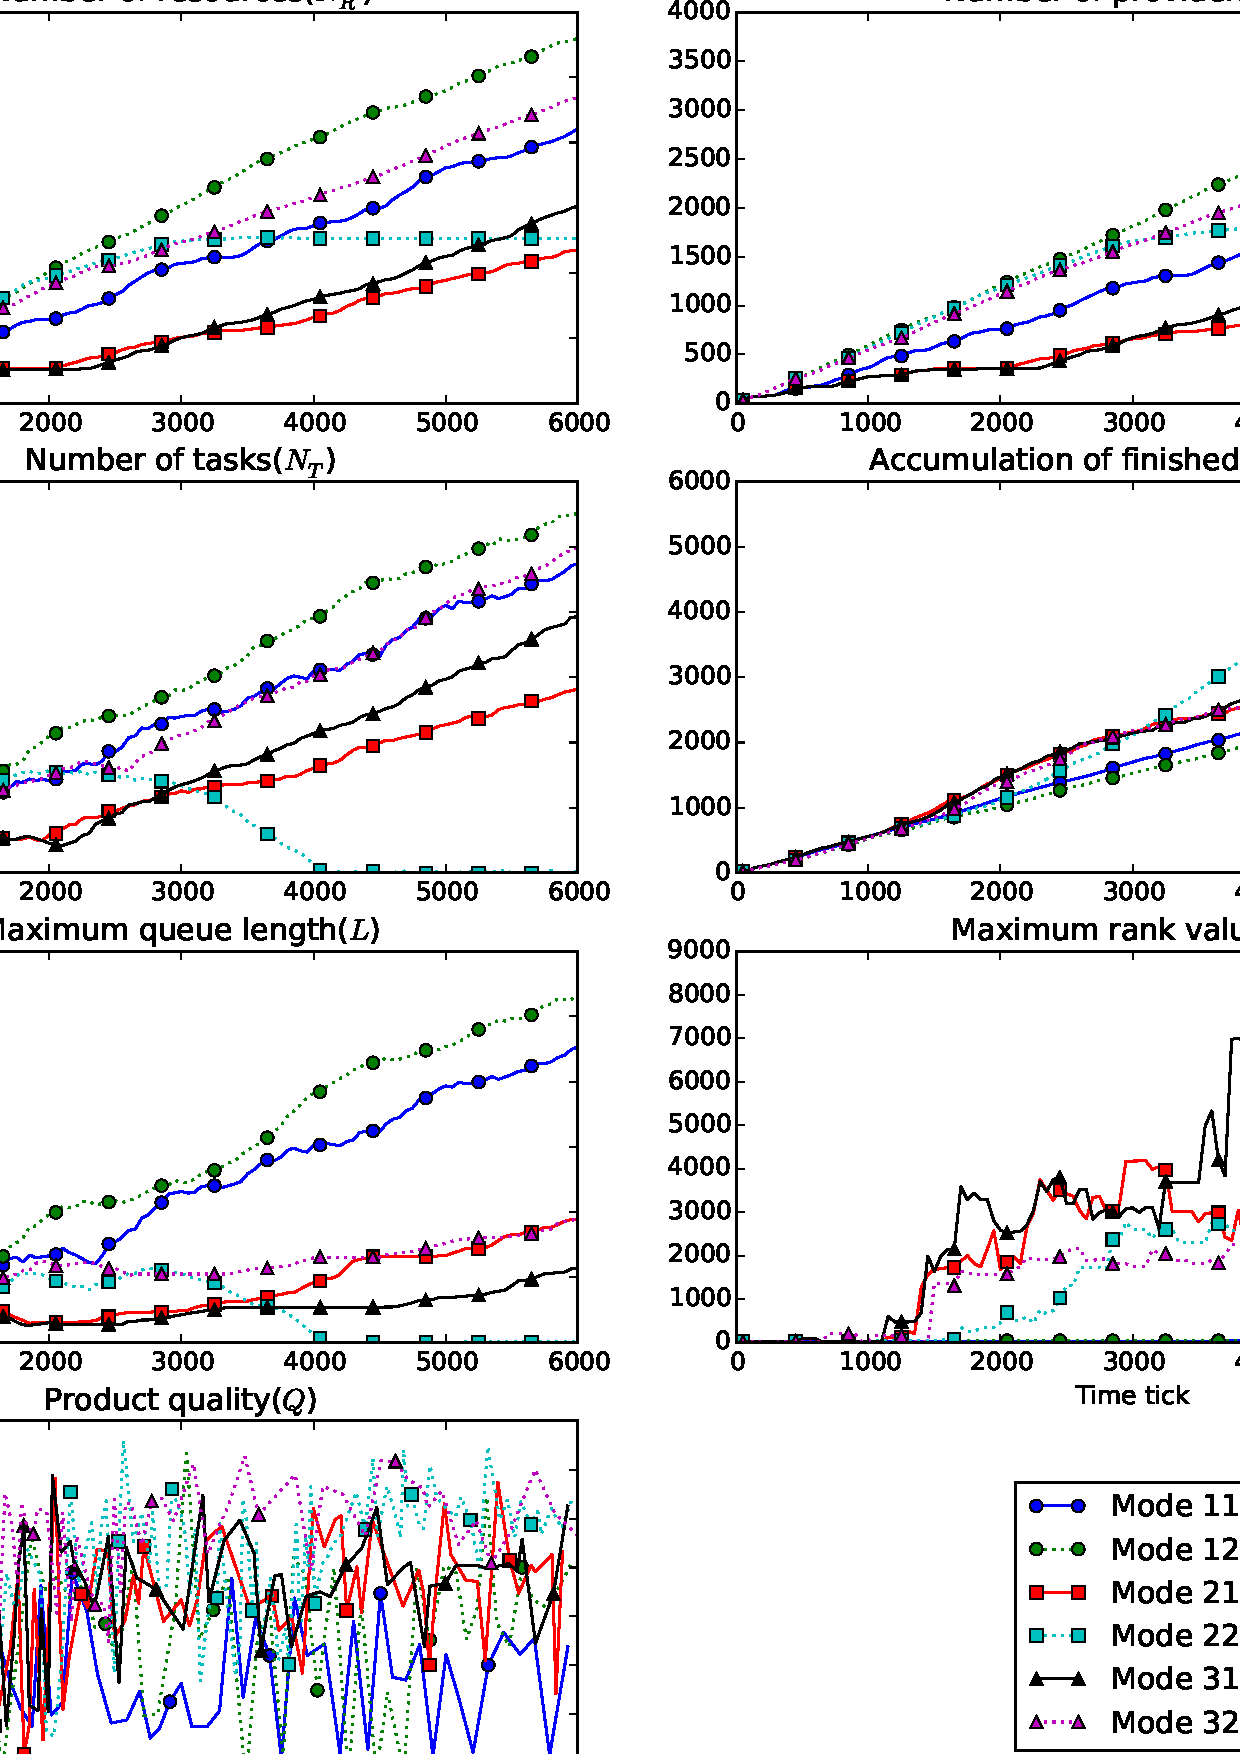
\includegraphics[width=\textwidth]{Data/out.pdf}
    \caption{Observed variable change with time}
    \label{fig:out}
\end{figure}
\begin{table}[htbp]
    \caption{Average observed values}
    \label{tab:averagevalue}
    \centering
    \scriptsize
    \begin{tabular}{lccccc}
    \toprule
    \textbf{Mode} & $\bar N_T$ & $\bar N_F$ & $\bar N_P$ & $\bar N_R $ & $\bar Q$\\
    \midrule
    Mode 11 & 1159.36 &  1644.201 &  1177.601 &  2053.727 &  8.388\\
    Mode 21 & \textit{636.769} &  \textit{2031.215} &  \textbf{692.716} &  \textbf{1066.947} &  16.016\\
    Mode 31 & 779.413 &  1996.021 &  \textit{782.272} &  \textit{1203.748} &  15.174\\
    Mode 12 & 1439.831 &  1522.923 &  1797.883 &  2954.113 &  14.057\\
    Mode 22 & \textbf{343.444} &  \textbf{2464.407} &  1316.952 &  1957.226 &  \textit{20.251}\\
    Mode 32 & 1164.409 &  1907.011 &  1597.742 &  2428.155 &  \textbf{20.652}\\

    \bottomrule
    \end{tabular}
\end{table}
we find: \begin{inparaenum}[1)]
\item Most dotted lines are above the full lines with the same series in $N_R,N_P,N_T$ means that metabolism mode need lower number of provider and resource, with the price of higher number of queue length of the tasks in resources in the system to deal with the same amount of needs, except for Mode 22, this combined mode even also need lower number of queue length. Full lines are not much above dotted lines in $N_F$ means that task processing velocity will be a little slower with the metabolism, exception also appears in Mode 22. 
\item $L$ and $N_T$ both represent the waiting of job, triangle and square line turned lower in $L$ meas that service-incubate mode can help reduce the waiting of job, these two type of line appeared above the circle line means the service-incubate mode do accelerate the processing velocity.
\item Triangle lines are a little above the square lines in $N_R,N_P,N_T$ means that outsource mode needs more resources to operate and can only reduce the waiting of job a little.
\item There is no big difference among all the 6 modes. Provider in metabolism mode will get lower rank value for they cannot stay in the system forever, the longer stay in the system, the higher rank value provider will get. Provider in Mode 11 even will not promote their rank value, which means that the metabolism rate is very fast without service-incubate mode.
\item Mode 22 is a very special mode that reached the balance of the system, although all the mentioned modes will reach balance in the long run, with the average data value shown in \autoref{tab:averagevalue}, metabolism with service-incubate but not with outsource mode is the easiest combine mode to maintain the system, resource are self configured and controlled to just meet the task need.
\end{inparaenum}

% subsubsection result_and_analysis (end)